%
% Copyright LANL
% Copyright Kitware
%
% This is documentation for the cinema file specification 
%

\documentclass{article}

\usepackage[export]{adjustbox}
\usepackage{authblk}
\usepackage[small,bf]{caption}
\usepackage{cite}
\usepackage{enumitem}
\setlist[description]{leftmargin=\parindent,labelindent=\parindent}
\usepackage{fancyhdr}
\usepackage{graphicx}
\usepackage[margin=1in]{geometry}
\usepackage{pdfpages}
\usepackage{tcolorbox}
\usepackage{times}
\usepackage{verbatim}
\usepackage{wallpaper}
\usepackage{xspace}
\usepackage{xcolor}


\begin{comment}
This is where we will put the copyright code
\end{comment}

\newcommand{\camstatic}     {\texttt{\small static}\xspace}
\newcommand{\camphi}        {\texttt{\small phi-theta}\xspace}
\newcommand{\cphi}          {\texttt{\small phi}\xspace}
\newcommand{\ctheta}        {\texttt{\small theta}\xspace}
\newcommand{\camazimuth}    {\texttt{\small azimuth-elevation-roll}\xspace}
\newcommand{\camyaw}        {\texttt{\small yaw-pitch-roll}\xspace}
\newcommand{\metadata}      {\texttt{\small metadata}\xspace}
\newcommand{\parameter}     {\texttt{\small parameter}\xspace}
\newcommand{\valuemode}     {\texttt{\small value\_mode}\xspace}
\newcommand{\namepattern}   {\texttt{\small name\_pattern}\xspace}
\newcommand{\pose}          {\texttt{\small pose}\xspace}
\newcommand{\parameterlist} {\texttt{\small parameter\_list}\xspace}
\newcommand{\cameramodel}   {\texttt{\small camera\_model}\xspace}

\newcommand{\LAUR} {LA-UR-17-20645\xspace}
\newcommand{\insitu} {\textit{in situ}\xspace}
\newcommand{\CinemaSpecVersion} {v1.0\xspace}
\newcommand{\Simple} {\textit{Simple}\xspace}
\newcommand{\chaplin} {Chaplin\xspace}
\newcommand{\cdevemail}{\texttt{\small cinema-dev@lanl.gov}\xspace} 
\newcommand{\cinemaemail}{\texttt{\small cinema@lanl.gov}\xspace} 
\pagestyle{fancy}
\fancyhf{}
\renewcommand{\headrulewidth}{0pt}
% \chead{\LAUR}
\cfoot{\thepage}

\newcommand{\todo}[1]{
}

%\newcommand{\todo}[1]{
    %\addcontentsline{tdo}{todo}{\protect{#1}}
    %\marginpar{\colorbox{white!90!black}{\textcolor{black}{
    %\parbox{2.1cm}{\scriptsize\bf\raggedright #1}
    %}}}
%}


\begin{document}

\renewcommand\Authands{ and }

% these lines implement subsubsubsection
\setcounter{secnumdepth}{5}
\setcounter{tocdepth}{5}
\newcommand{\subsubsubsection}[1]{\paragraph{#1}}


%---------------------------------------------------------------------
% Title page 
%---------------------------------------------------------------------
\ThisCenterWallPaper{1.0}{img/script_cover.png}
\thispagestyle{empty}

\begin{ttfamily}
\begin{center}
 \ \ \\
\vspace{1.0 in}
\begin{figure}[h!]
\centering

\includegraphics[height=0.5in]{img/cinema_logo_name}
\end{figure}
\vspace{1.0 in}
Cinema Database Specification \\
\chaplin Release v1.0\\
\bigskip
\begin{figure}[h!]
\centering

\includegraphics[height=1.0in]{img/chaplin_spec_logo}
\end{figure}
\bigskip
Document Version 1.4 \\
(31 January 2017)\\
\LAUR\\
\bigskip
\bigskip
\bigskip
\bigskip
by \\
\bigskip
David Rogers \texttt{\small dhr@lanl.gov}\\
Jon Woodring \texttt{\small woodring@lanl.gov}\\
John Patchett \texttt{\small patchett@lanl.gov}\\
David DeMarle \texttt{\small dave.demarle@kitware.com}\\
Berk Geveci \texttt{\small berk.geveci@lanl.gov}\\
\end{center}
\vspace{1.0 in}
\begin{flushright}
Los Alamos National Laboratory\\
Bikini Atoll Rd., SM 30\\
Los Alamos, NM 87545\\
cinema@lanl.gov\\
\end{flushright}
\end{ttfamily}
\newpage

\tableofcontents
\newpage

\pagenumbering{arabic}

%---------------------------------------------------------------------
% Begin Content
%---------------------------------------------------------------------

\section{Cinema Overview}
\label{sec:cinema}

Extreme scale scientific simulations are leading a charge to exascale computation, and data analytics runs the risk of being a bottleneck to scientific discovery. Due to power and I/O constraints, we expect in situ visualization and analysis will be a critical component of these workflows. 

Options for extreme scale data analysis are often presented as a stark contrast: write large files to disk for interactive, exploratory analysis, or perform in situ analysis to save detailed data about phenomena that a scientist knows about in advance. Cinema represents a novel framework for a third option – a highly interactive, data artifact-based approach that promotes exploration of simulation results, and is easily accessed through database specifications. This approach supports interactive exploration of a wide range of results, while still significantly reducing data movement and storage.

More information about the overall design of Cinema is available in the paper \textit{An Image-based Approach to Extreme Scale In Situ Visualization and Analysis} \cite{cinemaSC14}.

A Cinema Database supports the following three use cases. Taken together, these support a novel method for interactively exploring artifacts from extremely large datasets.

\begin{enumerate}
\item Searching/querying of meta-data and data artifacts. Samples can be searched purely on metadata, content, position, time, or a combination of all of these.
\item Interactive visualization of sets of data artifacts.
\item Playing interactive visualizations, allowing the user on/off control of elements in the visualization.
\end{enumerate}

\subsection{What is a Cinema Database?}
A Cinema database is a set of precomputed data artifacts that can be queried and interactively viewed. The user can decide what types of components comprise the database, based on the type of interaction that is desired with the final database.
A general design philosophy of Cinema is that applications reading and viewing a Cinema database can ignore data and determine which operations to perform. This promotes a wide range of possible interactions with the data - not just the ones imagined by the creator of the database.

Previous Cinema database specifications have concentrated on the notion that a database is a set of results sampled by visualization parameters. In this specification, we abstract this to include typical use cases from experiments by scientists. 

A scientist often has a spreadsheet with data about parameters for an experiment. This results in a set of parameters that map to a particular result - a graph, a sensor image, or other image-based data. These are a natural abstraction from previous Cinema databases. Figure \ref{fig:parametersets} shows this mapping of parameter sets to results. A collection of these mappings can be easily expressed in a Cinema database, using this specification. This is detailed in later sections.

\begin{figure}[h!]
\centering
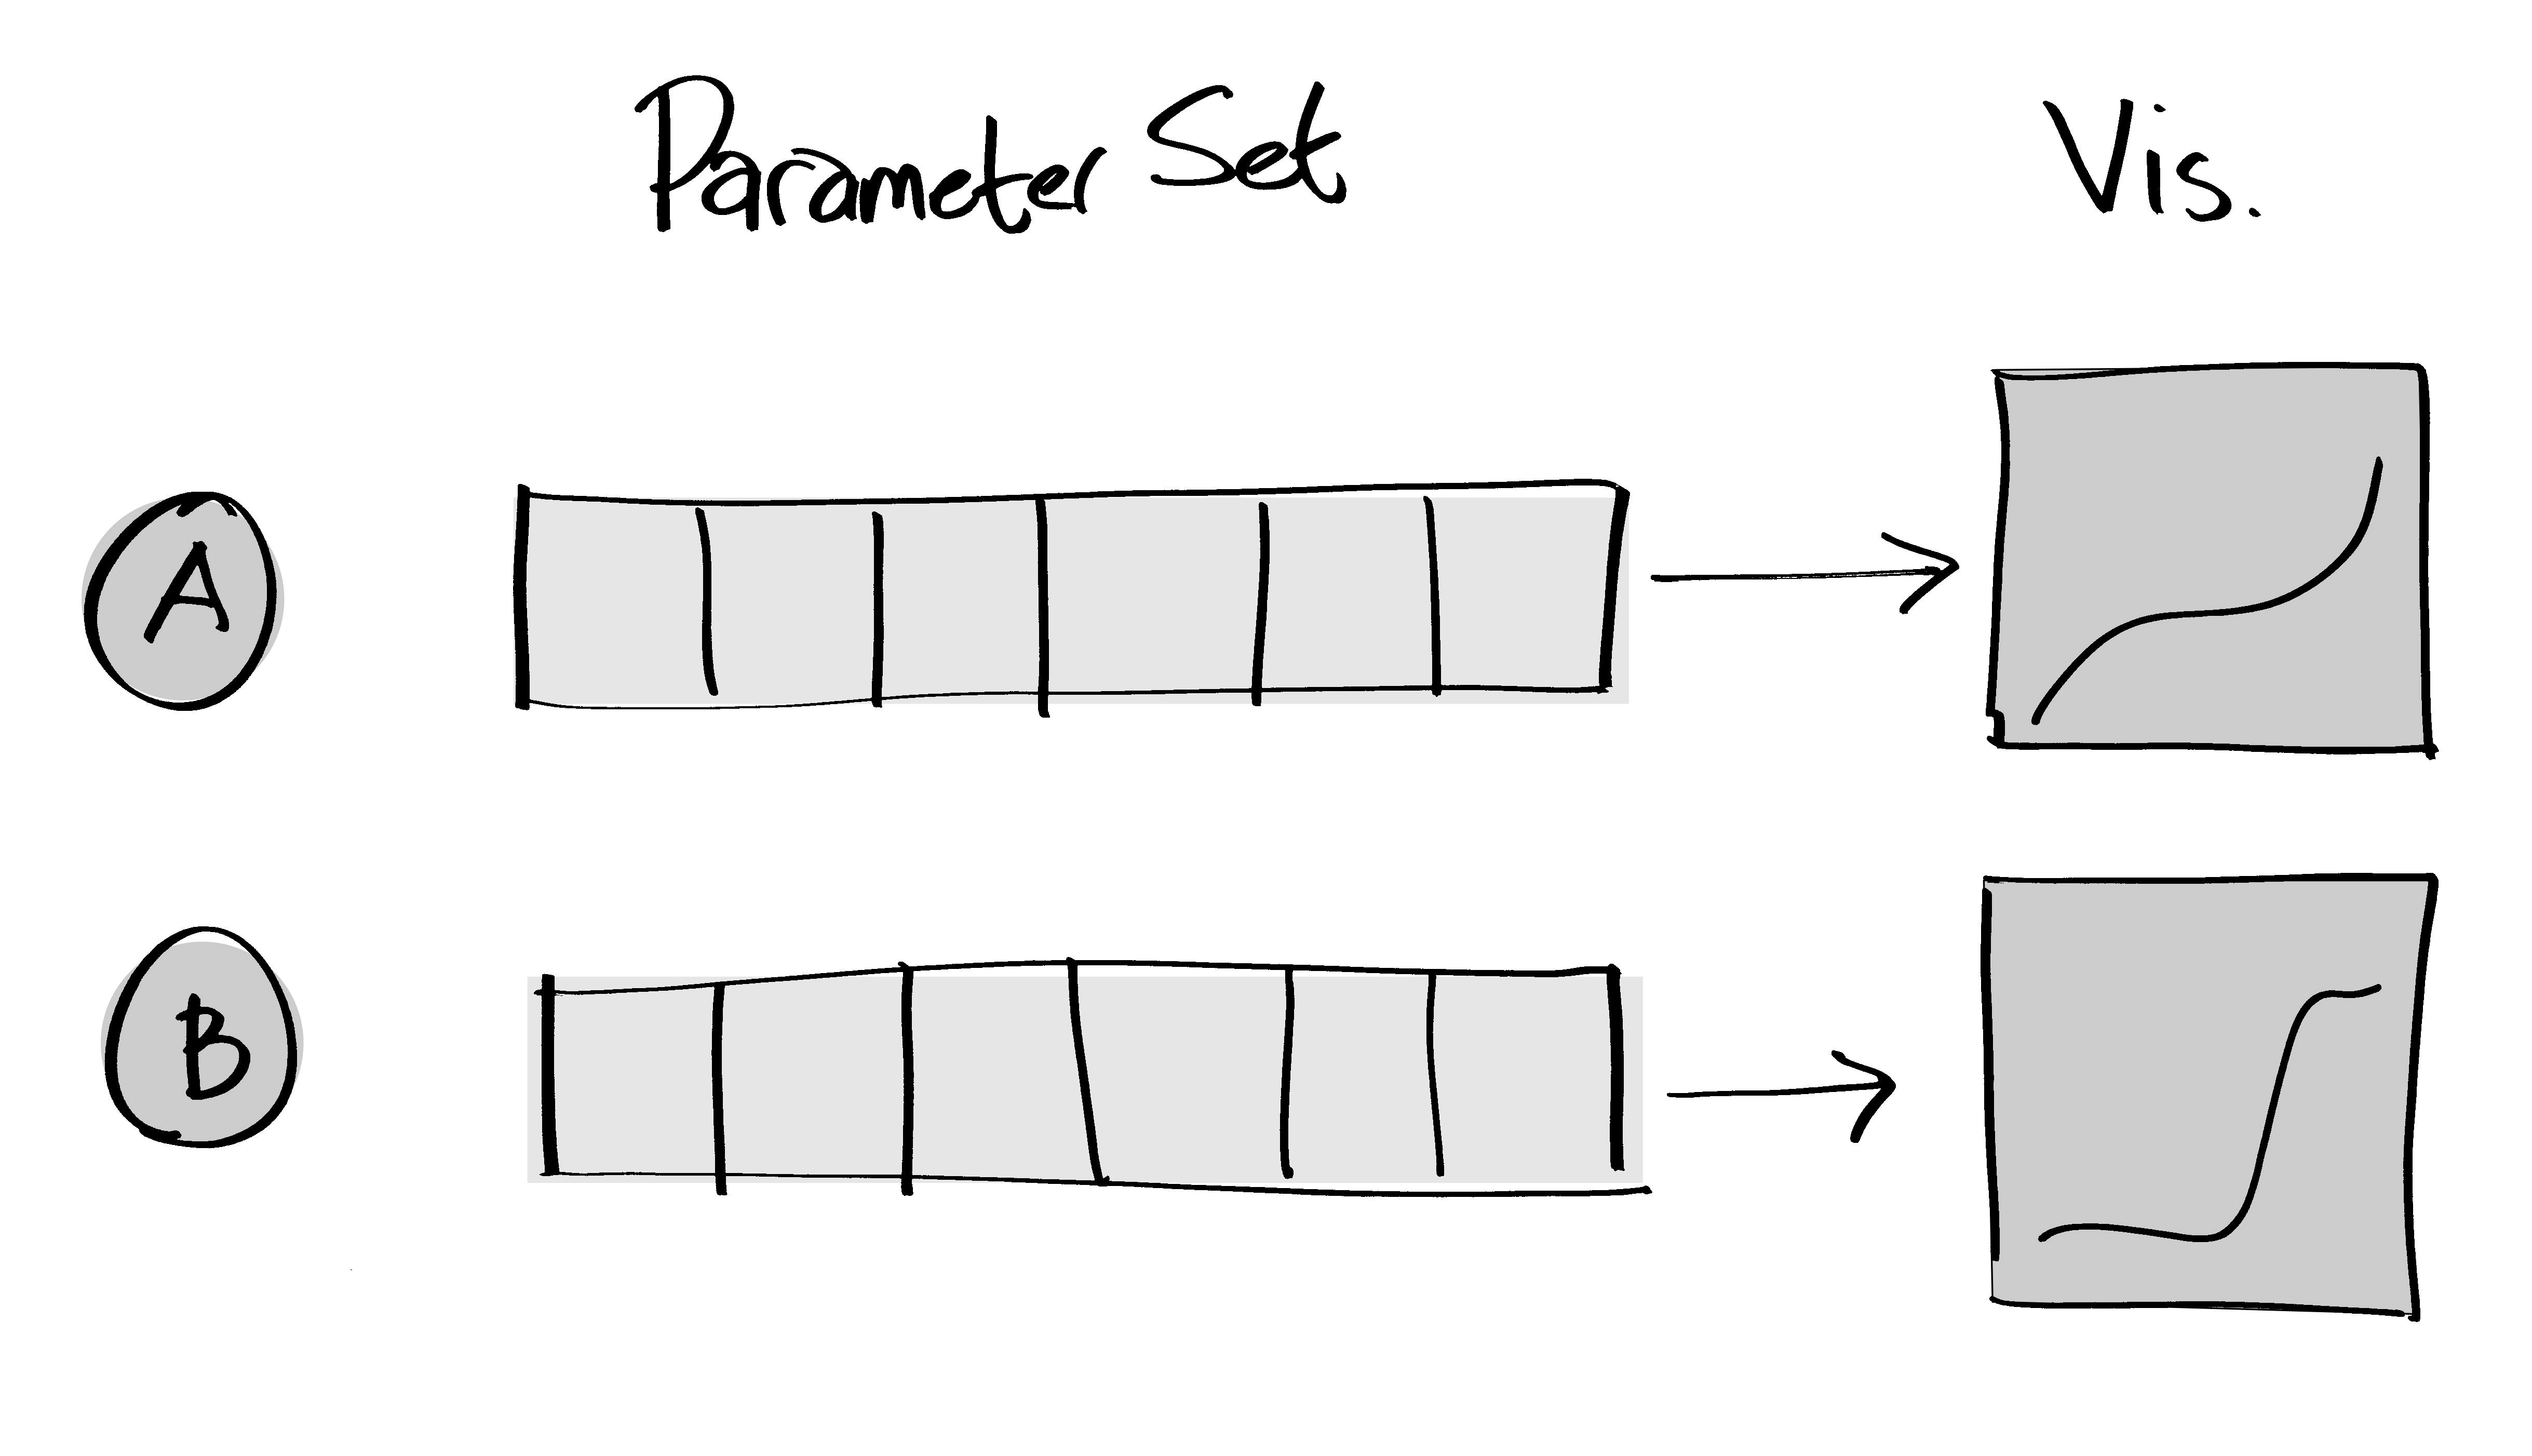
\includegraphics[width=0.8\textwidth]{img/parameter_set_diagram_filled}
\caption{
    Diagram showing a typical set of data that a scientist has for an experiment or simulations. Some set of parameters (A or B) has been used to create a visualization - a graph, an image captured from a sensor, or other data. These parameter sets can include, for example, settings on an experimental machine, inputs to a simulation, or measurements taken by a sensor. Each one of the parameter sets thus defines a unique result. Taken together, a set of these parameter sets constitutes a database of results, and a scientist often tracks this database in a spreadsheet. These parameter set/image pairings form the basis for the simplest Spec D database.
}
\label{fig:parametersets}
\end{figure}




\newpage
\section{The Cinema \chaplin Specification}
\label{sec:chaplin}

This document describes the Cinema \chaplin database so that collaborators can implement readers, writers, algorithms and viewers that perform different operations on Cinema databases. The document is broken into two main sections, one describing a \chaplin grammar, and one that describes the \chaplin implementation of that grammar. Applications and libraries that read and write databases that comply with both the grammar and the implementation in this document can expect to exchange, read and visualize data in a common format.

Subsections in the Grammar section (\ref{sec:grammar}) have corresponding sections in the Implementation section (\ref{sec:implementation}) of the document to fully explain the specification. There are several additional subsections in the Implementation section that provide file examples, and algorithms for mapping metadata to files on disc.

We invite public comment on this specification. Please send comments to \cdevemail.


\subsection{Chaplin Grammar}
\label{sec:grammar}

The base Chaplin
file, ``info.json'',
must adhere to the JSON standard, such that it can be parsed
by JSON readers.
Descriptive database elements are stored as 
JSON lists, objects (dictionaries), strings, and numbers.
To describe the grammar (syntax) for this file, we mostly follow 
from a typical Bachus-Naur form (BNF)-like/
Regular Expression (RE)-like conventions.
Certain grammar additions or deviations
from BNF and RE are explained below, which are intended
to shorten the description of the Chaplin grammar. 

The ``+''/``++'' and ``*'' repetition tokens are meant 
to represent a rule of a
repetition, as usual, but
with the convention that there is
a comma separating between each element
(i.e., it is shorthand for a comma
separated list, which is common in JSON). That is:
RULE+ or RULE++ means 
RULELIST ::= RULE , RULELIST $|$ RULE and
RULE* means EMPTYORRULELIST ::= ``'' $|$ RULELIST.
The ``++'' rule has an additional meaning that in its expansion,
each sub-rule must exist at least
once and only once (i.e., it is a list of unique
keys or key-value pairs that must be present).
The ``??'' token,  i.e., RULE??,
it means that rule is optional in a ``++'' production rule.
This means that that all right-hand elements that 
are produced from a ``RULE++'' are required to appear
at least once unless noted with a ``??''.
Furthermore, a ``??'' element is represented with $<$RULE$>$
on the left-hand side to further represent that it is optional.

To describe unique JSON values (keys), we introduce two
additions to the grammar specification.
KEY(NAME, SET) represents that a token, from a production
rule NAME, is added to a list SET during parsing,
where the list is named by the token generated by the rule SET.
The token generated by NAME must be
unique within that list SET (a specific token must appear only
once in its production
rule during parsing). REF(NAME, SET) means that
it is referring to a token within the list SET 
(a token may appear as many times as necessary
from a production rule during parsing,
but the specific token must exist in the list SET
as generated by KEY at the end of parsing).
If SET is the token ``global''
rather than a production rule, it means that the tokens generated
by KEY NAME are globally unique.  Otherwise,
it means that the tokens
generated by KEY NAME are ``scoped'' to a list, specifically
named by a token that is generated by the rule SET
(the list of unique tokens is the list named by SET).
Additionally, unique token production
rules are represented as \$NAME\$
on the left-hand side to indicate that they are meant to be unique.

JSONSTRING represents a valid JSON string, JSONNUMBER
represents a valid JSON number, and JSONVALUE
represents any valid JSON value, i.e., string, number, list, or dictionary.
``['' and ``]'' represent literal list enclosing elements for JSON,
rather than character range elements, such as typically used in 
RE notation. Likewise, ``\{'' and ``\}'' represent literal dictionary
enclosing brackets for JSON objects. 
``('', ``)'', and ``$|$'' represent
their typical RE expression meanings (groups and option).

\subsubsection{Top level}

As noted before, the Chaplin file must conform to JSON standards,
which contains nested dictionaries (objects). 
The top level anonymous JSON dictionary
must contain four elements that describe the contents
of a Chaplin database.

\begin{verbatim}
CHAPLIN ::= { TOP++ }
TOP ::= METADATADICT | NAMEPATTERNSTR | PARAMETERDICT | CONSTRAINTDICT 
\end{verbatim}

The four sub-sections are the metadata dictionary,
a name pattern string, parameter dictionary, and the constraint dictionary,
which are described further below.

\subsubsection{Metadata}

\begin{verbatim}
METADATADICT ::= "metadata" : { METADATA++ }
METADATA ::= DBTYPESTR | DBVERSIONNUM | STORETYPESTR | 
  CAMERAMODESTR | ENDIANSTR | IMAGESIZEPAIR |
  VALUEMODENUM?? | CAMERADATA?? | PIPELINELIST??  
\end{verbatim}

The metadata section is a collection of miscellaneous non-parametric
(input) information, such as database type and
version information, camera
information, output data format and size,
and a representation of the source generating 
data pipeline. It is further
described in section~\ref{sec:CONSTRAINTS}.

\begin{verbatim}
DBTYPESTR :: = "type" : 
  ("composite-image-stack" | "parameteric-image-stack")
DBVERSIONNUM :: = "version" : JSONNUMBER.JSONNUMBER
STORETYPESTR ::= "store_type" : ("FS" | "SFS")
CAMERATYPESTR ::= "camera_model" : ("static" | 
  "phi-theta" | "azimuth-elevation-roll" | "roll-pitch-yaw")
ENDIANSTR ::= "endian" : ("little" | "big")
IMAGESIZEPAIR ::= "image_size" : [ JSONNUMBER, JSONNUMBER ]
<VALUEMODENUM> ::= "value_mode": (1 | 2)
\end{verbatim}

At at minimum, the metadata requires the database type,
database version, storage type, camera model type, byte
endianness, and image size.
Value mode, the pipeline information, and camera information
are optional. The
pipeline information and camera information elements
are described further below.

\begin{verbatim}
<CAMERADDATA> ::= LOOK++
LOOK ::= EYELIST | ATLIST | UPLIST | NEARFARLIST | ANGLELIST
EYELIST ::= "camera_eye" : [ CARTESIAN3+ ]
ATLIST ::= "camera_at" : [ CARTESIAN3+ ]
UPLIST ::= "camera_up" : [ CARTESIAN3+ ]
NEARFARLIST ::= "camera_nearfar": [ NEARFARPAIR+ ]
ANGLELIST ::= "camera_angle": [ JSONNUMBER+ ]
CARTESIAN3 ::= [ JSONNUMBER, JSONNUMBER, JSONNUMBER ]
NEARFARPAIR ::= [ JSONNUMBER, JSONNUMBER ]
\end{verbatim}

The optional camera information is described by several
elements: the eye position list, looking at position list,
camera up list, the near-far plane list, and the 
vertical view angle (FOV) list.  

\begin{verbatim}
PIPELINELIST ::= "pipeline" : [ FILTERDICT+ ]
FILTERDICT ::= { FILTERDATA++ }
FILTERDATA ::= NAMESTR | IDNUM | VISNUM | PARENTLIST | CHILDRENLIST
NAMESTR ::= "name" : JSONSTRING
IDNUM ::= "id" : KEY(UUID, global)
$UUID$ ::= JSONNUMBER
VISNUM ::= "visibility" : (0 | 1)
PARENTLIST ::= "parents" : [ REF(UUID, global)* ]
CHILDRENLIST ::= "children" : [ REF(UUID, global)* ]
\end{verbatim}

The optional pipeline information is a description
of a set of filters (program objects)
that are connected together from inputs
to outputs in a directed acyclic graph (DAG).
These connections are
represented by parent and children relationships.
The ID value, UUID, is required to be a globally
unique number to identify each filter, in
the pipeline DAG. These IDs are referred to 
in the PARENTLIST and CHILDRENLIST, to create the DAG.

\subsubsection{Name Pattern}

\begin{verbatim}
NAMEPATTERNSTR ::= "name_pattern" : JSONSTRING
\end{verbatim}

The name pattern section describes
the default image channel file type and the file path for
image production. This primarily is used to locate
the image data channels on storage,
as described by the parameters.

\subsubsection{Parameters}

\begin{verbatim}
PARAMETERDICT ::= "parameter_list" : { PARAMETERDATADICT+ }
PARAMETERDATADICT ::= KEY(PARAMETERNAME, global) : { PARAMETERDATA++ } 
$PARAMETERNAME$ ::= JSONSTRING
PARAMETERDATA ::= LABELSTR | VALUELIST | DEFAULTVAL?? | 
  ROLESTR?? | VALUERANGEDICT?? | HINTSTR?? | CHANNELLIST??  
\end{verbatim}

The parameter section is the dictionary of changeable  
variables (independent,
input data). The database will contain,
on storage, image data channels.
These channels
are the result of the Cartesian product of parameters,
which generate
results (dependent, output data)
for every parameter value, except when a parameter is
constrained by another parameter value. 
PARAMETERNAME is the name of the parameter, which
is globally unique in the JSON file, and the right-hand
value is a dictionary containing the description
of that named parameter. 
Parameters are described fully in
section~\ref{sec:PARAMETERS}. 

\begin{verbatim}
LABELSTR ::= "label" : JSONSTRING
VALUELIST ::= "values" : [ (JSONVALUE | KEY(VALUENAME, PARAMETERNAME))+ ]
$VALUENAME$ ::= JSONSTRING
\end{verbatim}

At a minimum, the description of a
parameter requires a LABELSTR and VALUELIST.
If a VALUENAME key appears in VALUELIST
(a unique name per PARAMETERNAME of the parameter that VALUELIST
is contained in), 
it will be referenced
in VALUERANGEDICT to describe the value range of VALUENAME
for that PARAMETERNAME parameter.

\begin{verbatim}
<DEFAULTVAL> ::= "default" : JSONVALUE
<ROLESTR> ::= "role" : ("layer" | "control" | "field")
<VALUERANGEDICT> ::= "valuesRanges" : { RANGELIST+ }
RANGELIST ::= REF(VALUENAME, PARAMETERNAME) : [ JSONNUMBER, JSONNUMBER ] 
<HINTSTR> ::= "type" : ("hidden" | "range" | "option")
<CHANNELLIST> ::= "types" : [ CHANNELSTR+ ]
CHANNELSTR ::= "depth" | "luminance" | "value" | "color" | "lut"
\end{verbatim}

Parameter data have optional descriptors, DEFAULTVAL, ROLESTR,
VALUERANGEDICT, HINTSTR, and CHANNELLIST.
ROLESTR describes the primary use for this parameter.
VALUERANGEDICT entries are specific to
parameters that have a
ROLESTR of ``field'' to describe the value range of the parameter
(primarily to be used for color maps).
HINTSTR describes a hint for the how the parameter ought to be 
presented to the user.
CHANNELLIST is used to indicate the type of image
channels that are stored in the database for this parameter.

\subsubsection{Constraints}
\label{sec:g-constraints}

\begin{verbatim}
CONSTRAINTDICT ::= "constraints" : { CONSTRAINEDDICT+ }
CONSTRAINEDDICT ::= REF(PARAMETERNAME, global) : { VALIDLIST+ }
VALIDLIST ::= REF(PARAMETERNAME, global) : [ JSONVALUE+ ]
\end{verbatim}

The constraints section describes the relationships between variables
and how parameters are restricted by other parameter's
values. It is
described further
in section~\ref{sec:CONSTRAINTS}. Briefly, a
constrained parameter will be
ignored (not used to locate image data channels
on storage) whenever any of the listed valid parameters,
in VALIDLIST, have values outside of the listed set
(i.e., it is not used in the production of inputs
to outputs).



\newpage
\subsection{Chaplin Implementation}
\label{sec:implementation}

The content of a database is specified in a JSON format text file. The JSON file serves to enumerate the set of visualization samples, the relationships between them, and provides additional information used to interpret the content.

In any Cinema database, a number of different variables, or \textit{parameters} are of fundamental importance. Each parameter represents one setting that the user might vary to inspect the data with. Concrete examples include simulation time step, camera position, visibility, filter settings and choice of data array to color by.

In contrast to simpler Cinema databases, a \chaplin database contains a \textbf{subset} of the full combinatorial set of all variable settings. The contents are a subset because invalid and uninteresting combinations are excluded. Examples of excluded combinations are the color choice for a non-visible object and isolevel setting for data that is not being isocontoured.

As always, additional information about the database that is not of the same combinatorial visualization-space nature is useful. Examples of these include version numbers and time-dependent camera specific information.

The semantics and meaning of the four required top-level elements of the JSON file follow.


\subsubsection{Top level}
A valid \chaplin database has four sections in a JSON file: \texttt{\small metadata}, \texttt{\small name\_pattern}, \texttt{\small parameter\_list} and \texttt{\small constraints}. Details of the implementation are described in the following sections.


\subsubsection{Metadata}
\label{sec:metadata}

In addition to the sampled data as represented by the parameter space and constraint set, a cinema database contains additional data that describes the version of the database, supplemental information about cameras, and additional information about relationships between objects in the scene.

\subsubsubsection{Database Type (Required)}

The \textit{type} entry states whether this cinema store holds a \textit{Simple} non-compositable database, or a compositable database. Non-compositible databases have a value of ``parametric-image-stack''. These are described in the Astaire Specification document. Chaplin's compositible databases have a value of ``composite-image-stack''.

\begin{verbatim}
 "metadata": {
   "type": "composite-image-stack",
   ...
 },
\end{verbatim}

\subsubsubsection{Database Version (Required)}

A \textit{version} entry state the specific revision level within the type. The current revision level described in this document is 0.2.

\begin{verbatim}
 "metadata": {
   ...
   "version": "0.2",
   ...
 },
\end{verbatim}

\subsubsubsection{Store Type (Required)}

The \textit{store\_type} entry describes the lower level file format that the image channel data is kept in. It is possible to store the actual data under various containers. The one described in this document is implemented as named files within a filesystem directory as described in section~\ref{sec:storage}. The corresponding code is ``FS''  that is based on named files and directories. ``SFS'' is reserved for a storage format that places files within a VTK's XML image data volume files.

\begin{verbatim}
 "metadata": {
   ...
   "store_type": "FS",
   ...
 },
\end{verbatim}

\subsubsubsection{Camera Model (Required)}
\label{sec:cameramodel}

The camera model describes the camera behaviors encapsulated in the database. 
Cameras have different capabilities and constraints, and different supporting data is required for cameras in the \metadata and \parameter sections.  Supported models are:

\begin{itemize}
\item \camstatic This is a camera that looks at a fixed position. 
\item \camphi This corresponding to regularly sampled camera positions sitting on a ruled surface looking inward at a location in space. Requires \cphi and \ctheta parameters to define the angular samplings of the grid. This is described in Section~\ref{sec:camerapositions}.
\item \camazimuth This is an inward facing camera. Requires a \pose parameter to define the arbitrarily oriented normalized matrices that define the sampled camera directions. May optionally be supplemented with time varying offset location information about which the camera moves over time. This is described in the Section~\ref{sec:camerapositions}.
\item \camyaw This is an outward facing camera. 
Requires a \pose parameter to define the arbitrarily oriented normalized matrices that define the sampled camera directions. may optionally be supplemented with time varying offset location information about which the camera moves over time. This is described in the section~\ref{sec:camerapositions}.
\end{itemize}

\begin{verbatim}
 "metadata": {
   ...
   "camera_model": "azimuth-elevation-roll",
   ...
 },
\end{verbatim}

\subsubsubsection{Endian (Required)}
\label{sec:endian}

We store depth and value image channels as raw zlib compressed 32-bit
floating point files. The endian entry records the endianness that the
floats are stored in so that the underlying stream of bytes can be
correctly interpretted as numbers when read back in on a different computer.

\begin{verbatim}
 "metadata": {
   ...
   "endian": "little",
   ...
 },
\end{verbatim}

\subsubsubsection{Image Size (Required)}

We store depth and value image channels as raw zlib compressed 32-bit
floating point files. The image size entry records the width and height
of the data so that the underlying stream can be resized back
to the original rectangular shape when it is read back in.

\begin{verbatim}
 "metadata": {
   ...
   "image_size": [ 446, 955 ],
   ...
 },
\end{verbatim}

\subsubsubsection{Value Mode (Optional)}
\label{sec:valuemode}

This is a record of the type for value image channels. When the entry is absent, or contains the value ``1'', it means that the value image channels were made using the approximative method. Value images are floating point images in which each pixel is a number between 0.0 and 1.0 (the values are normalized) and then stored in a zlib compressed ``.Z'' file.

Note that if the \valuemode entry is present and contains the value ``2'' it means that the value images contain exact numerical quantities (the original data values) instead of normalized ones.

\begin{verbatim}
 "metadata": {
   ...
   "value_mode": 2,
   ...
 },
\end{verbatim}

\subsubsubsection{Camera Data (Optional)}
\label{sec:cameradata}

Supplemental camera information may be present to support the \camazimuth and 
\camyaw camera models. In either case cinema's parameter system provides an arbitrary list of camera directions. Those directions are placed at specific locations in space at each time step with the addition of offset information.

\begin{verbatim}
 "metadata": {
   "camera_model": "azimuth-elevation-roll",
   "camera_eye": [[0.0, 0.0, 66.92],  /*corresponds to time 0.0e+00*/
                  [1.0, 0.0, 66.92],  /*corresponds to time 1.0e-04*/
                  [2.0, 0.0, 66.92]], /*corresponds to time 8.0e-04*/
   "camera_at": [[0.0, 0.0, 0.0], /*as above */
                 [1.0, 0.0, 0.0],
                 [2.0, 0.0, 0.0]]
   "camera_up": [[0.0, 1.0, 0.0], /*as above */
                 [0.0, 1.0, 0.0],
                 [0.0, 1.0, 0.0]],
   ...
 }
\end{verbatim}

Furthermore, two additional optional pieces of information server to precisely define the viewing frustum at each sample. These are the camera\_nearfar and camera\_angle's.

\subsubsubsection{Pipeline (Optional)}

A pipeline entry directly encodes relationships between objects in the generating scene. It, in combination with the constraints and roles information is helpful for building up GUIs.

Here a graph of objects in the scene is explicitly recorded. This is not entirely redundant with the constraints system described in section~\ref{sec:CONSTRAINTS} because abstractly the later variable centric view is more inclusive and concretely because there is not generally a one to one relationship between objects and parameters. When objects are present the pipeline information facilitates organizing the controllable options to present them to the user.

\begin{verbatim}
 "metadata": {
   "pipeline": [
     { "children": [],
       "parents": [
         "2488"
       ],
       "id": "2687",
       "visibility": 1,
       "name": "Contour1" },
     { "children": [
         "2687"
       ],
       "parents": [
         "0"
       ],
       "id": "2488",
       "visibility": 1,
       "name": "Wavelet1" },
     ...
   ],
   ...,
 }
\end{verbatim}

\subsubsection{Name Pattern}
\label{sec:namepattern}

The \namepattern entry specifies the file format for RGB type color
component image channels (inluding 'color', 'lut' and 'luminance')
within the ``FS'' type database. The trailing file extension defines
this type. In comparison 'depth' and 'value' images are alwayed stored as zlib compressed
raw data in ``.Z'' files and thus do not need to be specified.

\begin{verbatim}
  "name_pattern": "{dontcare}.png",
\end{verbatim}


\subsubsection{Parameters}
\label{sec:PARAMETERS}

A \chaplin database is a collection of results sampled by a set of
visualization parameters. The collection of parameters that vary are
stored in the \parameterlist section of the json file.
Each parameter in the set is fully described by one of the
entries in the overall key-values pair. The values for each entry
contain information that together fully define the parameter,
including what is being sampled, the values it takes, and how the
results are to be interpretted. In \chaplin
everything from simulation time, to scene graph components, to operator
controls, to colors are represented by annotated parameters.

The pieces of information are stored within a dictionary within each paremeter.  The types of information are described
next. Examples of the most important parameters typically found in a
Cinema database follow them.

\subsubsubsection{Label (Required)}

Each parameter will have a label. This is a human readable string that
is intended to be presented to the user in a viewing application next to the
controls over the parameter.

\begin{verbatim}
  "parameter_list": {
    "parameter1": {
      "label": "slice plane offset",
      ...
\end{verbatim}

\subsubsubsection{Values (Required)}

Within the dictionary the most important element is a list of values
that the parameter takes on within the database.

\begin{verbatim}
  "parameter_list": {
    "parameter1": {
      ...
      "values": [ -0.5, -0.1, 0, 0.5, 42.0, 500.0 ],
      ...
\end{verbatim}

\subsubsubsection{Default Value (Optional)}

For viewing applications it is helpful to designate one entry within
the list of values as the default one to picked when the user has not
otherwise made a selection. If the default value is not written into
the file, the first entry in the list should be used instead.

\begin{verbatim}
  "parameter_list": {
    "parameter1": {
      ...
      "default": 42.0,
      ...
\end{verbatim}

\subsubsubsection{Role (Optional)}

Parameters may also have a \textit{role}. The roll more fully describes the
purpose of the parameter for generation and display purposes.

A role of ``layer'' indicates that this parameter defines what specific object or objects
should be shown. There is typically only one parameter with the role
in the database.  

\begin{verbatim}
  "parameter_list": {
    "vis": {
      "label": "objects in scene",
      "values": [
        "Slice1",
        "Superquadric1"
      ],
      "role": "layer"
      ...
    }
\end{verbatim}

A role of ``control'' indicates that this parameter is one of
a set that controls aspects of a specific object (i.e. filter
settings) and of the objects (i.e. downstream filters) that depend on it as well.

\begin{verbatim}
  "parameter_list": {
    "Slice1": {
      "label": "Slice1",
      "values": [ -0.5, 0.0, 0.5 ],
      "role": "control"
    },
\end{verbatim}

A role of ``field'' indicates that this parameter represents the set
of captured Image Channels for an object.

\begin{verbatim}
  "parameter_list": {
    "colorObject1": {
      "label": "Color Inputs for Object1",
      "values": [
        "depth",
        "Pressure_0",
        "Temperature_0"
      ],
      "types": [
        "depth",
        "lut",
        "lut"
      ],
      "role": "field"
    },
\end{verbatim}

For parameters with a role of ``field'' additional annotations (\textit{types} and \textit{valueRanges}) serve
to better specify the charactersitics of the Image Channels.

\subsubsubsection{Types -- Image Channels (Optional)}

\textit{types} is the mechanism by which the different channel types
are distinquished. It lists the specific image component type
corresponding to each entry in the field type parameter's value list. In the following
example we have three image channels, the first called ``depth'' is a
depth image. The second ``L'' is a luminance image. The last two channels
``pressure\_0'' and ``temperature\_0'' are value images.
 
\begin{verbatim}
  "parameter_list": {
    "colorObject": {
      "label": "color for a meteo result",
      "values": [
        "depth",
        "L",
        "pressure_0",
        "temperature_0"
      ],
      "role": "field",
      "types": [
        "depth",
        "luminance",
        "value",
        "value"
      ],
      ...
    },

\end{verbatim}

\subsubsubsection{Value Range (Optional)}

For value type image channels it is useful to record the minimum and
maximum recorded values for the corresponding data array or
arrays. The value range annotation does this within a dictionary of
names to minimum and maximum value pairs. For every ``value'' type image channel, there will be a
corresponding entry in the value range dictionary. Continuing the
above example we add storage for the range of both the pressure
and temperature data.

\begin{verbatim}
  "parameter_list": {
    "colorObject": {
      "label": "color for a meteo result",
      "values": [
        "depth",
        "L",
        "pressure_0",
        "temperature_0"
      ],
      "role": "field",
      "types": [
        "depth",
        "luminance",
        "value",
        "value"
      ],
      "valueRanges": {
        "pressure_0": [ 29.4, 29.8 ],
        "temperature_0": [33.0, 36.5 ]
      },
      ...
    },
\end{verbatim}

\subsubsubsection{Display Hint (Optional)}

Parameters may have a suggested widget \textit{type}. The type is used as
a hint for viewing applications to inform what type of GUI widget is most
appropriate for this control. A type of ``option''
is best displayed with a combobox type widget that lets the user select many
values at once. A type of ``range'' is best displayed with a menu,
scalar bar, or slider, that lets the user select just one value
at any give time time.  A type of ``hidden'' should generally not be
displayed to the user.

\begin{verbatim}
  "parameter_list": {
    "vis": {
      "label": "vis",
      "role": "layer",
      "type": "option",
      ...
    "slice": {
      "label": "slice plane offset",
      "role": "control",
      "type": "range",
      ...
    "color": {
      "label": "color channels",
      "role": "field",
      "type": "hidden",
      ...
     }
\end{verbatim}

\subsubsubsection{Parameter Example: Time}
\label{sec:Time}

Time varying data can be sampled at arbitrary points along the temporal domain.
\begin{verbatim}
 "parameter_list": {
   "time": { "default": "0.000000e+00",
             "values": ["0.000000e+00", "1.000737e-04", "1.999051e-04"],
             "type": "range",
             "label": "simulation time" },
   ...
 }
\end{verbatim}

\subsubsubsection{Parameter Example: Camera Positions}
\label{sec:camerapositions}

In a traditional visualization setting the user can manipulate the camera arbitrarily. For cinema we discretize and organize the range of captured motions into of several camera motion classes. 
The camera model in use within a database is listed in the \cameramodel
entry of the json files metadata section. 
See section~\ref{sec:cameramodel} for specifics. 

\begin{itemize}
\item \camstatic No addition information needed in this section. 
Static cameras do not require a corresponding parameter entry.

\item \camphi A model in which the discrete camera positions are described by the product of two parameters with angular positions. Additional information needed defines the \cphi and \ctheta values. The camera ``from'' position varies over a set of regularly sampled angular positions centered around a chosen focal point. These cameras will have one or two corresponding parameters entries. In Cinema, \cphi is defined to be rotations around the vertical axis, going from -180 to 180 degrees, inclusive on the negative only. \ctheta is defined to be rotations from south to north pole, ranging from -90 to 90 degrees inclusive.
\begin{verbatim}
 "parameter_list": {
   "phi": { "default": -180,
            "values": [-180, -150, -120, -90, -60, -30,
                       0,
                       30, 60, 90, 120, 150],
            "type": "range",
            "label": "phi" },
   "theta": { "default": -90,
              "values": [-90, -64, -38, -12, 13, 38, 63, 88],
              "type": "range",
              "label": "theta" },
   ...
 }
\end{verbatim}
\item \camyaw and \camazimuth both require a \pose section. 
In these more general \pose based cameras, we store complete camera reference frames from an arbitrary collection of viewpoints. 

These cameras require a \pose parameter, which contains any number of 3x3 normalized camera reference frames. To keep the combination of camera positions over time and view directions manageable, we vary the camera's local coordinate frame consistently at every time step, but offset them from a different location at each time step. An example is shown below. 
\begin{verbatim}
 "parameter_list": {
  "time": {
    "values": ["0.0e+00",
               "1.0e-04",
               "8.0e-04"],
     ... },
  "pose": {
    "values": [[[-1.0, 1.224e-16, 7.498e-33],
                [0.0, 6.123e-17, -1.0],
                [-1.224e-16, -1.0, -6.123e-17]],
               [[-1.0, 1.109e-16, 5.175e-17],
                [0.0, 0.422, -0.906],
                [-1.224e-16, -0.906, -0.422]],
               ... ],
    ...
    },
  ...
 }
\end{verbatim}
\end{itemize}

\subsubsubsection{Parameter Example: Objects}
\label{sec:objects}

Different items may be displayed in the scene. During image generation
it is important that only one object be displayed at a time so that we
can capture its depth, color, value and other image channels in
isolation. From the viewing application the end user selects zero or
more entries from the same parameter to show any number of objects
together at the same time. Visibility parameters have a \textit{role} annotation of ``layer''.

\begin{verbatim}
 "parameter_list": {
   "vis": {
     "values": [
       "Contour1",
       "Wavelet1",
       ...
     ],
     "role": "layer",
     "type": "option",
     ...
   }
 }
\end{verbatim}

\subsubsubsection{Parameter Example: Operators}
\label{sec:operators}

Zero or more operators, such as clipping plane and isocontour samples along with their respective ranges are represented by parameters. Operators, like other parameters are cumulative. For each operator, the value is applied and the resulting scene is recorded. Operator parameters have a \textit{role} annotation of ``control''.

\begin{verbatim}
 "parameter_list": {
    "Contour1": {
      "values": [37.3531, 97.2221, 157.091, 216.96, 276.829],
      "role": "control",
      ...
    },
    ...
 }
\end{verbatim}

\subsubsubsection{Parameter Example: Output Image Channels}
\label{sec:image_channels}

In a Cinema workflow, the application producing a Cinema Database creates a set of image channels for each sample in the parameter space. Viewing applications use these channels to draw objects and to color them dynamically dependent on the user's choices for solid color or colormapped value arrays. Recall that ``types'' and ``valueRanges'' annotations are important for interpreting the output of each possible value for a color control.

The types entries describe the specific image channels type. There are several possible image channels.

\begin{itemize}
\item \textbf{Required}. One of the following image channels is required. Both \textbf{cannot} be present.
\begin{itemize}
\item \textbf{RBG}. An image containing colored pixel information. This can be one of two types:
\begin{itemize}
\item \textbf{Color} channel. This encodes a standard RGB value for each pixel - the result of rendering the viewpoint from the camera. 
Color images can not be dynamically color mapped.
\item \textbf{LUT (Lookup Table)} channel. This contains pixels that have been colored by applying a colormap to a single variable.
\end{itemize}
\item \textbf{Value} channel. This encodes an arbitrary array value associated with the data that is visualized at each pixel. Global ranges for each array, i.e. the min and max value for a value over all time steps and parameter settings, are recorded in the meta data file. In \chaplin, value images are stored as floating point image channels, where the value is either normalized between 0.0 and 1.0 or kept unmodified, and stored in a ``.Z'' file. This is described more fully in section~\ref{sec:valuemode}.
\end{itemize}
\item \textbf{Optional}. These channels enable other types of operations.
\begin{itemize}
\item \textbf{Depth} channel. This encodes a depth value for every pixel, relative to the camera. Required for compositing. In \chaplin, depth images are stored as floating point image channels, ranging from 0 for the near plane to 255 for the far plane, and kept in zlib compressed ``.Z'' files. As with value images the word size is 32bit. The endianness and image dimensions are recorded in the metadata section's endian and image\_size entries.
\item \textbf{Luminance} channel. This encodes a rendered shading brightness for each pixel. Required for lighting to be included in the final rendering. In \chaplin, luminance images are stored in RGB images where the R component contains the ambient gray value, G contains the diffuse, and B contains the specular component. Of these, currently only the diffuse component is used. All components range from 0 to 255.
\end{itemize}
\end{itemize}

An example of this parameter list section follows. Here we have all possibilities for the image channels of an object named ``Contour1''. The image channels consist of depth, luminance, and a value for a scalar quantity called ``RTData''. The RTData array varies over the entire simulation and for all objects between 37 and 277.

\begin{verbatim}
 "parameter_list": {
   "colorContour1": { 
     "values": ["depth", "luminance", "RTData_0"],
     "types": ["depth", "luminance", "value"],
     "valueRanges": {"RTData_0": [37.3531, 276.829]},
     "role": "field"
   },
   ...
  }
\end{verbatim}



\subsubsection{Constraints}
\label{sec:CONSTRAINTS}

Constraints are relationships between parameters. These are included in the specification because a visualization is sometimes designed so that parameters are constrained by and dependent on others. For example, a visualization might include two unrelated objects with different sets of arrays on each object. In such a scene, the choice of what array to use to apply colors then depends on what object is displayed.

% A generating application must visit all reachable states to produce results and it must avoid visiting and storing results for invalid and redundant states. A viewing application must ensure that all values that affect the appearance of an object are taken into account when deciding what contents are required for display.

% These relationships turn otherwise order independent options into a graph of parent child relationships. Unconstrained parameters will be fully sampled within the database. Constrained parameters will be sampled fully whenever at least one of its constraints are met.

In cinema we store this information in a constraints entry in the json file. It consists of a list of parameters, and for each parameter in the list there is a sub list of one or more parameters and associated parameter values, that the containing parameter's presence depends upon. See section~\ref{sec:g-constraints}.

A specific example of this with an object's color inputs are only output when the vis layer parameter shows that the object is selected. Likewise for the color of the contour object.

\begin{verbatim}
 "constraints": {
    "colorContour1": {
      "vis": [
        "Contour1"
      ]
    },
    "colorObject1": {
      "vis": [
        "Object1"
      ]
    },
    ...
\end{verbatim}


A more complicated example which adds in two levels of dependencies is as follows. Here we represent a the three element data pipeline that might create a visualization. In the pipeline a Sphere object is fed into a Slice filter and the Slice filter is fed into a Clip filter.

\begin{verbatim}
 "constraints": {
    "colorSphere1": {
      "vis": [
        "Sphere1"
      ]
    },
    "colorSlice1": {
      "vis": [
        "Slice1"
      ]
    },
    "colorClip1": {
      "vis": [
        "Clip1"
      ]
    },
    "Sphere1": {
      "vis": [
        "Clip1",
        "Sphere1",
        "Slice1"
      ]
    },
    "Slice1": {
      "vis": [
        "Clip1",
        "Slice1"
      ]
    }
    "Clip1": {
      "vis": [
        "Clip1"
      ]
    },
    ...
\end{verbatim}

To begin with there is the color relationship information described above. Besides that there is information about the parameters for objects along the pipeline.

Starting at the end of the pipeline the clipping plane value is sampled whenever the clipped data is shown. Going one step up the pipeline the slice plane's value must be varied whenever either the slice or the clip output are visible. This is necessary because the slice filter is an input to the clip filter so its value affects the appearence of the clipped result. Likewise hypothetical parameters of the sphere object itself (the radius for example) have to vary whenever any of the three objects were visible. Remember also that if the visibility parameter selects something other than one of these three objects, then none of these parameters will be exercised.


\subsubsection{Storage Structure}
\label{sec:storage}

A low level data storage layer beneath the metadata layer holds individual results in the form of image channels saved as images. For example, a depth image channel for one particular object drawn from one particular viewpoint at one particular time step. For each valid combination of parameter settings, their will be one file.

The storage layer organizes results into numbered directories within a tree hierarchy. Each directory corresponds to a variable and numbered contents correspond to different values for the variable. The mapping of numbers to data values comes from the list of values for each parameter in the metadata. In the example below we have a data base with two time steps, each with two camera poses and two objects. The first object has three color components, the second has only two.

\begin{verbatim}
results/
  info.json
  pose=0/
    time=0/
      vis=0/
        color=0.Z
        color=1.png
        color=2.Z
      vis=1/
        color=0.Z
        color=1.png
    time=0/
      vis=0/
        color=0.Z
        color=1.png
        color=2.Z
      vis=1/
        color=0.Z
        color=1.png
  pose=1/
    time=0/
      vis=0/
        color=0.Z
        color=1.png
        color=2.Z
      vis=1/
        color=0.Z
        color=1.png
    time=1/
      vis=0/
        color=0.Z
        color=1.png
        color=2.Z
      vis=1/
        color=0.Z
        color=1.png
\end{verbatim}

\begin{comment}
The directory hierarchy follows an order that satisfies the constraints between variables. Applications that use the cinema python reference library should not worry about the specific layout of the results as they will be be isolated from version incompatibilities by the reference library. They can simply use the libraries MongoDB like database API to search for, insert and retrieve contents based on parameter names and values. For applications that can not use the reference API, the exact file structure mapping is described below.

This information is provided for those who wish to bypass the cinema\_python reference library but still use or create compatible file stores. In this situation it is necessary to know exactly how to map parameter value combinations to file names. There are three important aspects, one is to derive the file type and file format extension, another is to derive a specific file name for a particular value, and the last is to derive a consistent directory path given a collection of values.

Note that the exact format of the store has changed over time as Cinema has evolved. The reference library uses a cinema store's included version markers to provide backwards compatibility. We here describe the latest version information as of Cinema Chaplin version 0.1. For further details consult the FileStore class's \_get\_filename() method in the reference library.
\end{comment}

\subsubsubsection{Constructing a Path to Output Files}

The scheme we use to consistently arrange files into the file system is to sort alphabetically the parameter names, and then lay out the data in sub-directories in a dependency following order. In particular parameters with no dependencies go first, and then as dependencies are satisfied, dependent parameters follow, always within alphabetical order at each dependency level.

A pseudocode summary of the standard implementation's \_get\_filename() method
of the file\_store class is as follows.
\begin{verbatim}
        keys = [sort(parameters_names)]
        ordered = []
        while len(keys):
            k = keys.pop(0)
            parents = k.getdependees()
            ready = all parents already in ordered
            if not ready:
                keys.append(k) # try back later
            else:
                ordered.append(k) # this one is next
        for k in ordered:
            index = offset for parameter[k]'s value
            filename = filename + "/" + key + "=" + index
\end{verbatim}


With parameters:
\begin{verbatim}
"b_param": {"values": [1,-2]}
"a_param": {"values": ["a","b"]}
"c_param": {"values": [42.0, 3.1415926535897932384626433832795028841971],
            "types": ["depth","rgb"],
            "role": "field" }
"d_param": {"values": ["I","II","III"],
            "types": ["luminance","value","depth"],
            "role": "field"}
\end{verbatim}
and constraints:
\begin{verbatim}
constraints": {
   "c_param": {
      "b_param": [1]
   },
   "d_param": {
      "b_param": [-2],
   }
}
\end{verbatim}

and filename\_pattern ``dontcare.tiff'':
the resulting layout would be:
\begin{verbatim}
  a_param=0/b_param=0/c_param=0.Z
  a_param=0/b_param=0/c_param=1.tiff
  a_param=0/b_param=1/d_param=0.tiff
  a_param=0/b_param=1/d_param=1.Z
  a_param=0/b_param=1/d_param=2.Z
  a_param=1/b_param=0/c_param=0.Z
  a_param=1/b_param=0/c_param=1.tiff
  a_param=1/b_param=1/d_param=0.tiff
  a_param=1/b_param=1/d_param=1.Z
  a_param=1/b_param=1/d_param=2.Z
\end{verbatim}

Because ``a\_param'' comes before ``b\_param'' alphabetically. ``c\_param'' and ``d\_param'' follow their shared dependee ``b\_param'' and would do so even if they were renamed to something less than ``b\_param''.

Adding another dependency level would change the layout with the new parameter following its own dependee.
\begin{verbatim}
"aa_param": {"values": [10, 11]}
\end{verbatim}
additional constraint:
\begin{verbatim}
   "aa_param": {
      "d_param": ["I","III"]
   }
\end{verbatim}
\begin{verbatim}
  a_param=0/b_param=0/c_param=0.Z
  a_param=0/b_param=0/c_param=1.tiff
  a_param=0/b_param=1/d_param=0/aa_param=0.tiff
  a_param=0/b_param=1/d_param=0/aa_param=1.tiff
  a_param=0/b_param=1/d_param=1.Z
  a_param=0/b_param=1/d_param=2/aa_param=0.Z
  a_param=0/b_param=1/d_param=2/aa_param=1.Z
  a_param=1/b_param=0/c_param=0.Z
  a_param=1/b_param=0/c_param=1.tiff
  a_param=1/b_param=1/d_param=0/aa_param=0.tiff
  a_param=1/b_param=1/d_param=0/aa_param=1.tiff
  a_param=1/b_param=1/d_param=1.Z
  a_param=1/b_param=1/d_param=2/aa_param_0.Z
  a_param=1/b_param=1/d_param=2/aa_param_1.Z
\end{verbatim}

\subsubsubsection{File Type}

There are a variety of content types in a \chaplin store: depth and value images are files of floating point numbers, while luminance and color images are files of RGB tuples. The content type is determined from a ``field'' or color parameter's  ``types'' entry. For each value that one of these parameters takes, the corresponding ``types'' entry indicates if it is 'rgb', 'depth', 'value', or 'luminance' type content.

\begin{verbatim}
 "parameter_list": {
   "colorContour1": { "values": ["val1", "val2", "val3"],
                      "types": ["depth", "luminance", "value"],
                      "valueRanges": {"RTData_0": [37.3531, 276.829]},
                      "role": "field" },
   ...
  }
\end{verbatim}

In the example above, whenever the colorContour1 parameter takes on ``val1'', the content is a depth image. When it is ``val2'' the content is a luminance image. When it is ``val3'' it is a value image. In \chaplin depth and value images are stored in zlib compressed ``.Z'' files. Everything else is stored in a standard image format. The choice of a specific image format, ``.png'', ``.tiff'', ``.jpeg'' and the like is made based on the trailing file extension from the \textit{name\_pattern} entry.

\subsubsubsection{File Name}

Parameter settings are encoded into file and directory names. We use a ``key=index'' scheme for all parameters where the key is the parameter name and the index is the 0 based index into the values list to a specific value. In the example above when colorContour1 parameter takes on ``val1'' the result will appear in a file or directory named ``colorContour1=0''. Using indices instead of values avoids a number of conversion problems involving decimal precision and also the fact that non-scalar values do not map well onto file system naming rules.


\newpage
\subsubsection{Single Database Example}
\subsubsubsection{JSON file}

This example is based on the above JSON schema outline.                 

\begin{verbatim}
{
  "metadata": {
    "type": "composite-image-stack",
    "version": "0.2",
    "store_type": "FS",
    "image_size": [ 446, 955 ],
    "endian": "little",
    "value_mode": 2,
    "camera_model": "azimuth-elevation-roll",
    "camera_eye": [
      [ -0.023820051408253964, 1.3749762463487758, 2.409604270242429 ]
    ],
    "camera_at": [
      [ 0.0, 0.0, 0.0 ]
    ],
    "camera_up": [
      [ 0.003238554846559421, 0.8685535085368621, -0.49558482076311905 ]
    ],
    "camera_nearfar": [
      [ 0.007973907729484015, 7.973907729484015 ]
    ],
    "camera_angle": [
      30.0
    ],
    "pipeline": [
      {
        "children": [],
        "parents": [ "3970" ],
        "id": "4254",
        "visibility": 1,
        "name": "Slice1"
      },
      {
        "children": [ "4254" ],
        "parents": [ "0" ],
        "id": "3970",
        "visibility": 1,
        "name": "Superquadric1"
      }
    ]
  },
  "name_pattern": "{pose}.png",
  "parameter_list": {
    "colorSlice1": {
      "types": [
        "depth",
        "luminance",
        "value",
        "value"
      ],
      "type": "hidden",
      "role": "field",
      "valueRanges": {
        "TextureCoords_0": [ 0.0, 1.0 ],
        "TextureCoords_1": [ -0.0017080907709896564, 1.0 ]
      },
      "values": [
        "depth",
        "luminance",
        "TextureCoords_1",
        "TextureCoords_0"
      ],
      "label": "colorSlice1",
      "default": "TextureCoords_0"
    },
    "Slice1": {
      "label": "Slice1",
      "type": "hidden",
      "role": "control",
      "values": [ -0.5, 0, 0.5 ],
      "default": -0.5
    },
    "pose": {
      "label": "pose",
      "type": "range",
      "values": [
        [[1.0, 0.0, 7.498798913309288e-33],
         [7.498798913309288e-33, -6.123233995736766e-17, -1.0],
         [0.0, 1.0, -6.123233995736766e-17]],
        [[1.0, 1.2246467991473532e-16, 1.2246467991473532e-16],
         [1.2246467991473532e-16, -1.0, 0.0],
         [1.2246467991473532e-16, 1.4997597826618576e-32, -1.0]],
        [[-1.0, -1.2246467991473532e-16, 0.0],
         [1.2246467991473532e-16, -1.0, 0.0],
         [0.0, 0.0, 1.0]],
        [[1.0, 2.4492935982947064e-16, 7.498798913309288e-33],
         [7.498798913309288e-33, -6.123233995736766e-17, 1.0],
         [2.4492935982947064e-16, -1.0, -6.123233995736766e-17]],
        [[-1.0, 1.2246467991473532e-16, 7.498798913309288e-33],
         [0.0, 6.123233995736766e-17, -1.0],
         [-1.2246467991473532e-16, -1.0, -6.123233995736766e-17]],
        [[-1.0, 0.0, 1.2246467991473532e-16],
         [0.0, 1.0, 0.0],
         [-1.2246467991473532e-16, 0.0, -1.0]],
        [[1.0, 0.0, 0.0],
         [0.0, 1.0, 0.0],
         [0.0, 0.0, 1.0]],
        [[-1.0, -1.2246467991473532e-16, 7.498798913309288e-33],
         [0.0, 6.123233995736766e-17, 1.0],
         [-1.2246467991473532e-16, 1.0, -6.123233995736766e-17]]],
      "default": [
         [1.0, 0.0, 0.0],
         [0.0, 1.0, 0.0],
         [0.0, 0.0, 1.0]
       ]
    },
    "colorSuperquadric1": {
      "types": [
        "depth",
        "luminance",
        "value",
        "value"
      ],
      "type": "hidden",
      "role": "field",
      "valueRanges": {
        "TextureCoords_0": [ 0.0, 1.0 ],
        "TextureCoords_1": [-0.0017080907709896564, 1.0 ]
      },
      "values": [
        "depth",
        "luminance",
        "TextureCoords_1",
        "TextureCoords_0"
      ],
      "label": "colorSuperquadric1",
      "default": "TextureCoords_0"
    },
    "vis": {
      "label": "vis",
      "type": "option",
      "role": "layer",
      "values": [
        "Slice1",
        "Superquadric1"
      ],
      "default": "Slice1"
    }
  },
  "constraints": {
    "colorSlice1": {
      "vis": [
        "Slice1"
      ]
    },
    "Slice1": {
      "vis": [
        "Slice1"
      ]
    },
    "colorSuperquadric1": {
      "vis": [
        "Superquadric1"
      ]
    },
    "Superquadric1": {
      "vis": [
        "Slice1",
        "Superquadric1"
      ]
    }
  }
}
\end{verbatim}

\subsubsubsection{Associated File Structure}

Using the above example, the following paths would be expected for the resulting image channels:

\begin{verbatim}
./info.json
./pose=0/vis=0/Slice1=0/colorSlice1=0.Z
./pose=0/vis=0/Slice1=0/colorSlice1=1.png
./pose=0/vis=0/Slice1=0/colorSlice1=2.Z
./pose=0/vis=0/Slice1=0/colorSlice1=3.Z
./pose=0/vis=0/Slice1=1/colorSlice1=0.Z
./pose=0/vis=0/Slice1=1/colorSlice1=1.png
./pose=0/vis=0/Slice1=1/colorSlice1=2.Z
./pose=0/vis=0/Slice1=1/colorSlice1=3.Z
./pose=0/vis=0/Slice1=2/colorSlice1=0.Z
./pose=0/vis=0/Slice1=2/colorSlice1=1.png
./pose=0/vis=0/Slice1=2/colorSlice1=2.Z
./pose=0/vis=0/Slice1=2/colorSlice1=3.Z
./pose=0/vis=1/colorSuperquadric1=0.Z
./pose=0/vis=1/colorSuperquadric1=1.png
./pose=0/vis=1/colorSuperquadric1=2.Z
./pose=0/vis=1/colorSuperquadric1=3.Z
./pose=1/vis=0/Slice1=0/colorSlice1=0.Z
./pose=1/vis=0/Slice1=0/colorSlice1=1.png
...
./pose=6/vis=1/colorSuperquadric1=2.Z
./pose=6/vis=1/colorSuperquadric1=3.Z
./pose=7/vis=0/Slice1=0/colorSlice1=0.Z
./pose=7/vis=0/Slice1=0/colorSlice1=1.png
./pose=7/vis=0/Slice1=0/colorSlice1=2.Z
./pose=7/vis=0/Slice1=0/colorSlice1=3.Z
./pose=7/vis=0/Slice1=1/colorSlice1=0.Z
./pose=7/vis=0/Slice1=1/colorSlice1=1.png
./pose=7/vis=0/Slice1=1/colorSlice1=2.Z
./pose=7/vis=0/Slice1=1/colorSlice1=3.Z
./pose=7/vis=0/Slice1=2/colorSlice1=0.Z
./pose=7/vis=0/Slice1=2/colorSlice1=1.png
./pose=7/vis=0/Slice1=2/colorSlice1=2.Z
./pose=7/vis=0/Slice1=2/colorSlice1=3.Z
./pose=7/vis=1/colorSuperquadric1=0.Z
./pose=7/vis=1/colorSuperquadric1=1.png
./pose=7/vis=1/colorSuperquadric1=2.Z
./pose=7/vis=1/colorSuperquadric1=3.Z

\end{verbatim}


\subsubsection{Combining Multiple Databases}
\label{sec:multiview}

It is often convenient to group cinema data bases together. This is useful, for example in the case of multi-view applications. In this case, independent databases can be collected as siblings in a higher level directory, and another json file which lists the directories can provide information about the set.

An example directory hierarchy containing the above and corresponding json file follow.

\begin{verbatim}
collection.cdb/
  info.json
  results/
    info.json /*etc as above*/
  moreresults/
    info.json /*similar to above*/
\end{verbatim}

The top level info.json here would be as follows.

\begin{verbatim}
{
  "metadata": {
    "type": "workbench"
  },
  "runs": [
    { "title": "a view of some data",
      "description": "interesting results ...",
      "path": "results" },
    { "title": "a different view",
      "description": "even more interesting results ...",
      "path": "moreresults" }
  ]
}
\end{verbatim}


\section{Notes on Previous Specifications}
The Cinema project updates specifications as new capabilities are integrated into the overall design. Specifications are named in alphabetical order.

\begin{itemize}
\item \textit{Astaire} is currently supported. The specification is available on the Cinema website \texttt{\small www.cinemascience.org}.
\item \textit{Bacall} has been deprecated. 
\item \textit{Chaplin} is this specification.
\end{itemize}


\section{Contact Information}
There are a lot of ways to get in touch with us. First, you can contact the authors of this document. In addition:

\begin{itemize}
\item Developer mailing list: \cdevemail.
\item General Cinema mailing list: \cinemaemail.
\item Cinema website: \texttt{\small cinemascience.org}. This includes documentation, specifications, examples and applications (viewers, etc.)
\item Cinema website: \texttt{\small cinemaviewer.org}. This site shows several examples of browser-based cinema viewers with various scientific databases. 
\end{itemize}



\bibliography{bib}{}
\bibliographystyle{unsrt}


\end{document}
